As mentioned before, we add the Jastrow term to form the second trail wave function Eqt. \ref{eq:t2}.
Moreover, in this situation, we have two variational parameters $\alpha$ and $\beta$.
It largely increases our computing time.

This time, we still start from $\omega=1$ and $N=10^7$ and vary $\alpha$ from 0.675 to 1.15, $\beta$ from 0.1 to 0.3.
Here, it will be cumbersome to show all energies and variances.
So we only present a Fig. \ref{fig:t2} to give an intuitive impression.
\begin{figure}[tb]
\label{fig:t2}
\centering
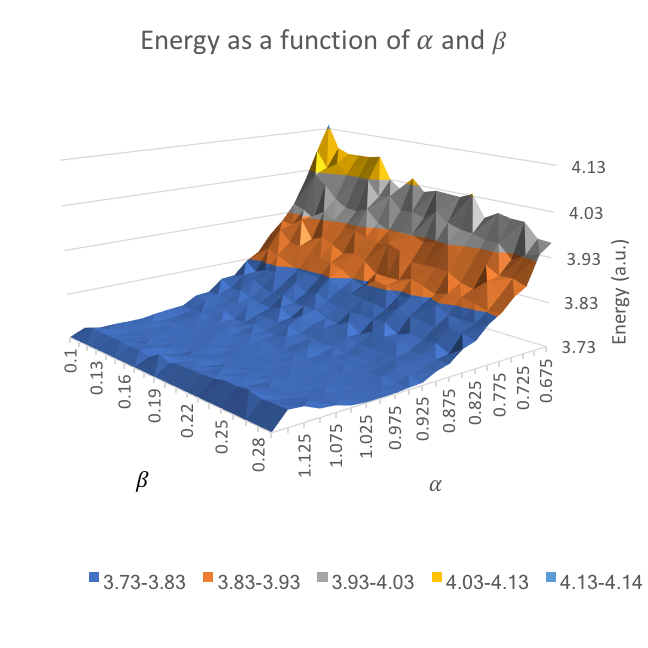
\includegraphics[width=0.4\textwidth]{t2.png}
\caption{Relation between lowest $E$(a.u.) and the variational parameters $\alpha$ and $\beta$ where $\omega$ is set to one and $N=10^7$ obtained from $\Phi_{t2}$.}
\end{figure}
The lowest energy is $E_{min}=3.7305\ a.u.$ with parameters $\alpha=1.025$ and $\beta=0.18$.
The $r_{12}$ obtained from $\Phi_{t2}$ are listed in the third column of Table \ref{tab:t12}.
We can see the values are larger than the second column (from $\Phi_{t1}$).
It is reasonable because $\Phi_{t1}$ doesn't take Coulomb repulsion into account in the wave function.
It then underestimates the distance $r_{12}$.

In project 2, we also solve the ground state energy of this system by diagonalizing its Hamiltonian.
It gives a rather accurate results for this system.
So we use it as a standard benchmark of results obtained from MC method.
\begin{table}[tb]
	\centering
	\caption{Minimum energies calculated from two trail wave functions (second and third columns) and diagonalization method (fourth column). Optimal parameter used with $\omega=0.01,0.5$ and 1.0, $N=10^7$. All qualities are in atomic unit.}
	\label{tab:diag}
	\begin{tabular}{cccc}
		\hline
		\hline
		$\omega$   &$E_{min}(t1)$ & $E_{min}(t2)$ & $E_{min}(diag)$ \\
		\hline
		0.01 &0.104 &0.0935 &0.0796  \\
		0.50 &2.0394 &2.0005 &1.99995  \\
		1.00 &3.7729 &3.7305 &3.72992 \\
		\hline
		\hline
	\end{tabular}
\end{table}
Their results are shown in Table \ref{tab:diag}.
We can see both second and third columns obtained by MC method for two different trail wave functions  reproduce results from diagonalization method.
Deviations are larger for $\omega \neq 1$ because we keep using optimal parameters for $\omega=1$ which is not the best for other .
Furthermore, $\Phi_{t2}$ gives smaller error than $\Phi_{t1}$ which means the Jastrow factor makes it more similar to exact the wave function.
